\documentclass[sigconf]{acmart}
\setcopyright{none}
\settopmatter{printacmref=false,printfolios=false}
\renewcommand\footnotetextcopyrightpermission[1]{}
\acmDOI{}
\acmISBN{}
\acmConference{}{}{}
\pagestyle{plain}
\fancyhead{}
\usepackage{booktabs}
\usepackage{tabularx}
\usepackage{multicol}
\usepackage{listings}
\usepackage{xcolor}
\usepackage{iftex}
\ifXeTeX\setmonofont{Inconsolatazi4}[Extension=.otf,UprightFont=*-Regular,BoldFont=*-Bold,Scale=1]\fi
\lstdefinelanguage{SPARQL}{morekeywords={SELECT,FROM,WHERE,FILTER,NOT,EXISTS,GROUP,BY,ORDER,AS,COUNT,INSERT,DATA,DELETE,GRAPH,WITH,OPTIONAL,a,CONTAINS,LCASE},sensitive=true,alsoletter={?},morestring=[b]"}
\lstset{language=SPARQL,basicstyle=\ttfamily\scriptsize,keywordstyle=\bfseries,breaklines=true,columns=fullflexible,keepspaces=true,showstringspaces=false,aboveskip=3pt,belowskip=3pt}
\newcommand{\repolink}{\url{https://github.com/MohamedKhalidmk/TRIAD}}
\newcommand{\tw}[1]{\texttt{#1}}

\begin{document}
\setlength{\emergencystretch}{1em}
\title{TRIAD: A Knowledge Graph of Clinical Assertions}
\titlenote{Code, ontology, knowledge-graph scripts, setup instructions, license and artificial intelligence (AI) review log: \repolink.}
\author{Asish A. George}
\affiliation{\institution{University of Victoria}\city{Victoria}\state{BC}\country{Canada}}
\email{asishgeorge@uvic.ca}
\author{Mohamed Khaled}
\affiliation{\institution{University of Victoria}\city{Victoria}\state{BC}\country{Canada}}
\email{mabuela@uvic.ca}

\begin{abstract}
A clinical chart must tell a correction from a contradiction: who said what, when, and which claim replaced which. In Milestone~4 we stored this in 29 SQLite relations, where every fact is an assertion that may supersede an earlier one. We now map the same entity-relationship (ER) model to a Web Ontology Language (OWL~2) ontology with 28 classes, 25 object and 92 datatype properties, and 18 keys, and we map the relational data to a knowledge graph of 1,298,482 Resource Description Framework (RDF) triples with the RDB-to-RDF Mapping Language (R2RML). The same application runs on SQLite, Oxigraph and Virtuoso, and all 16 of our Structured Query Language (SQL) queries return the same rows in the SPARQL Protocol and RDF Query Language (SPARQL). Code: \repolink.
\end{abstract}

\keywords{Semantic Web, OWL 2, R2RML, SPARQL, SHACL, provenance}
\maketitle

\section{Problem Definition}
In 2019 a patient tells the front desk she had a rash after penicillin, and the medical office assistant (MOA) records an allergy; in 2024 another clinic's record repeats it; in 2026 a test is negative and the doctor rules it out. A chart of values still shows the allergy. TRIAD stores each claim as an \emph{assertion} in a \emph{message} with an issuer and a time, and a new assertion \emph{supersedes} the one it corrects.

\textbf{Information need.} For every clinical entry, return the current assertion (the one nothing supersedes), its author and message, and the chain it replaced. We answer it from a knowledge graph in OWL~2~\cite{owl2}, aligned to the PROV Ontology (PROV-O)~\cite{provo} and to Fast Healthcare Interoperability Resources (FHIR) R4~\cite{fhir-r4}.

\section{From ER and Relations to an Ontology}\label{sec:onto}
A script checks our Turtle ontology against the SQL schema and writes \tw{triad.owl} (RDF/XML, 1,956 triples). Page~3 gives the mapping (Figure~\ref{fig:onto}).
{\sloppy\setlength{\leftmargini}{1em}\begin{itemize}\setlength{\itemsep}{0pt}
\item \textbf{Entity sets} become 23 classes, \textbf{M:N relationships with attributes} 3 association classes (\tw{WorksIn}, \tw{VisitLocation}, \tw{Citation}), and \textbf{multivalued composite attributes} 2 value classes: 28 classes for 29 relations, since \tw{StaffLanguage} becomes the multivalued property \tw{language}.
\item \textbf{Rows} become individuals named by class path and surrogate key (\tw{kg:assertion/3}); \textbf{attributes} become 92 datatype properties, 91 functional. NOT NULL gives \tw{owl:minCardinality 1}; the 17 \tw{CHECK \dots\ IN} lists become closed ranges (\tw{owl:oneOf}).
\item \textbf{Foreign keys} become 17 stored object properties in the ER direction (\tw{issues}, \tw{contains}, \tw{about}, \tw{supersedes}, \dots), with \tw{owl:cardinality 1} where the key is mandatory, and 5 named inverses. The one-to-one \tw{supersedes} is functional, inverse-functional, asymmetric and irreflexive.
\item \textbf{IS-A} becomes \tw{rdfs:subClassOf} with \tw{owl:disjointUnionOf}. A subtype row is the \emph{same} individual as its parent row (\tw{kg:staff/2 a triad:Staff, triad:Nurse}), so the discriminator columns need no property.
\item \textbf{Keys} become 18 \tw{owl:hasKey} axioms; a weak entity's key uses its owner's inverse, \tw{Assertion hasKey (inMessage seq)}.
\item {\raggedright \textbf{Paths} become 3 derived properties: \tw{ofPatient} = \tw{about}$\circ$\tw{during}$\circ$\tw{visitOf}, \tw{assertedBy} = \tw{inMessage}$\circ$\tw{issuedBy}, and the transitive \tw{supersedesTransitively}.\par}
\end{itemize}}

\textbf{What OWL cannot hold.} Under the Open World Assumption (OWA), OWL describes knowledge and rejects no data: a missing NOT NULL value is unknown, not an error. ``Current'' means ``no newer assertion'', which OWL cannot state, so each query writes \tw{FILTER NOT EXISTS}. A key is worse: Milestone~4 identifies a patient by (Name, DateOfBirth), and two different patients with the same name and birthday would make a reasoner infer \tw{owl:sameAs} and merge them, with no error. So the rules moved (see \tw{ontology.md}): 29 Shapes Constraint Language (SHACL)~\cite{shacl} node shapes with 28 SHACL-SPARQL constraints, 24 SPARQL checks, and guards in the app that refuse a write (409 or 422). One rule is new, not converted: a staff member must work in a department.

\textbf{Reasoning.} In Protégé~5.6, HermiT~\cite{hermit} finds the ontology consistent, with no unsatisfiable class. With the seed graph imported, it finishes with no error and infers \tw{assertedBy} for all 10 seed assertions (Description Logic, DL, query \tw{'asserted by' some Staff}). It skips the 31 \tw{xsd:date} values of the seed graph, which OWL~2 lacks; HermiT run through owlready2 stops on them.

\section{The Knowledge Graph}\label{sec:kg}
An R2RML~\cite{r2rml} mapping of 35 TriplesMaps, run by Morph-KGC~\cite{morphkgc}, turns the Milestone~4 database (113 patients, 5,090 visits, 57,022 assertions; Synthea~\cite{synthea} data and our own bundle) into 1,298,482 triples: 188,271 \tw{rdf:type}, 911,697 attribute and 198,514 foreign-key triples about 130,959 individuals. The ontology and the data go into the named graphs \tw{\dots/tbox} and \tw{\dots/abox}. Unlike the World Wide Web Consortium (W3C) Direct Mapping~\cite{directmapping}, which turns one Assertion row into 14 triples with string times and a literal for every key, ours gives 10, with typed times and one object property per foreign key. Virtuoso~7.2~\cite{virtuoso} serves it in Docker; Oxigraph runs embedded.

\section{SPARQL Operations}\label{sec:ops}
Six SPARQL~1.1~\cite{sparql11} scripts mirror the SQL ones; our \tw{03\_\allowbreak select\_\allowbreak queries.sparql} holds Q1--Q14b in full. Prefixes are omitted; \tw{\dots} shortens Internationalized Resource Identifiers (IRIs).

\textbf{Q1, what is true now}, joins patient, visit, entry, assertion and message, and keeps each assertion with \tw{FILTER NOT EXISTS \{ ?n triad:supersedes ?a \}} (8 rows); the issuer is \tw{OPTIONAL}, as a patient's own message has none. \textbf{Q2, the revision chain.} Milestone~4 needed a recursive \tw{WITH}; SPARQL has no recursion, but the property path \tw{supersedes*} walks the chain from the current assertion. The depth of each assertion is the number of nodes between it and the head:
\par\noindent\begin{minipage}{\columnwidth}\begin{lstlisting}
SELECT ((COUNT(?mid) - 1) AS ?depth) ?date ?author ?statement
FROM <.../abox>
WHERE { ... ?e a triad:Allergy ; triad:substance ?s .
  FILTER (CONTAINS(LCASE(?s), "penicillin"))
  ?head triad:about ?e .
  FILTER NOT EXISTS { ?n triad:supersedes ?head }
  ?head triad:supersedes* ?mid . ?mid triad:supersedes* ?a .
  ... }
GROUP BY ?a ?date ?author ?statement ORDER BY ?depth
\end{lstlisting}\end{minipage}\par
\noindent It returns the same three rows as the recursive common table expression (CTE) of Milestone~4, on all three stores:
\par\noindent{\scriptsize\setlength{\tabcolsep}{3pt}\begin{tabularx}{\columnwidth}{@{}rlllX@{}}
\toprule
\textbf{depth} & \textbf{date} & \textbf{author} & \textbf{origin} & \textbf{statement}\\
\midrule
0 & 2026-10-02 & A. Okafor (Doctor) & Staff & Not allergic. Test negative.\\
1 & 2024-03-05 & S. Alvarez (MOA) & OtherClinic & Penicillin allergy (copied from \dots).\\
2 & 2019-06-12 & S. Alvarez (MOA) & Patient & Patient report: rash after penicillin \dots\\
\bottomrule
\end{tabularx}}\par

\textbf{Insert, update and delete.} \tw{INSERT DATA} adds a patient; an update is \tw{DELETE/INSERT \dots\ WHERE} (SPARQL has no \tw{UPDATE}), with the old value \tw{OPTIONAL}:
\par\noindent\begin{minipage}{\columnwidth}\begin{lstlisting}
INSERT DATA { GRAPH <.../abox> { <.../kg/patient/900001>
  a triad:Patient ; triad:name "Noah Fielding" ;
  triad:dateOfBirth "1990-03-14"^^xsd:date . } }

WITH <.../abox>
DELETE { ?p triad:phoneNumber ?old }
INSERT { ?p triad:phoneNumber "+1-508-555-0199" }
WHERE { ?p a triad:Patient ; triad:name "Elena Marsh" ;
        triad:dateOfBirth "1971-05-14"^^xsd:date .
        OPTIONAL { ?p triad:phoneNumber ?old } }
\end{lstlisting}\end{minipage}\par
\noindent A delete keeps the foreign-key rule by hand: it removes a patient only if \tw{FILTER NOT EXISTS \{ ?s triad:hasVisit ?v \}}. Users do not write SPARQL: the app's forms add, search, update and delete, and the \emph{Delete patient} form shows this refusal (Figure~\ref{fig:ui}). A clinical fact is never changed in place; a correction is a new superseding assertion.

\textbf{SQL = SPARQL.} A test checks that all 16 queries give the same rows on SQLite, Oxigraph and Virtuoso. The stores differ where the standard does not: Virtuoso orders a stored \tw{xsd:\allowbreak dateTime} by its text, finds \tw{sameTerm} false for equal IRIs, and runs the updates of one request without a transaction. Failing tests found 10 such quirks.

\begin{figure}[t]
\centering
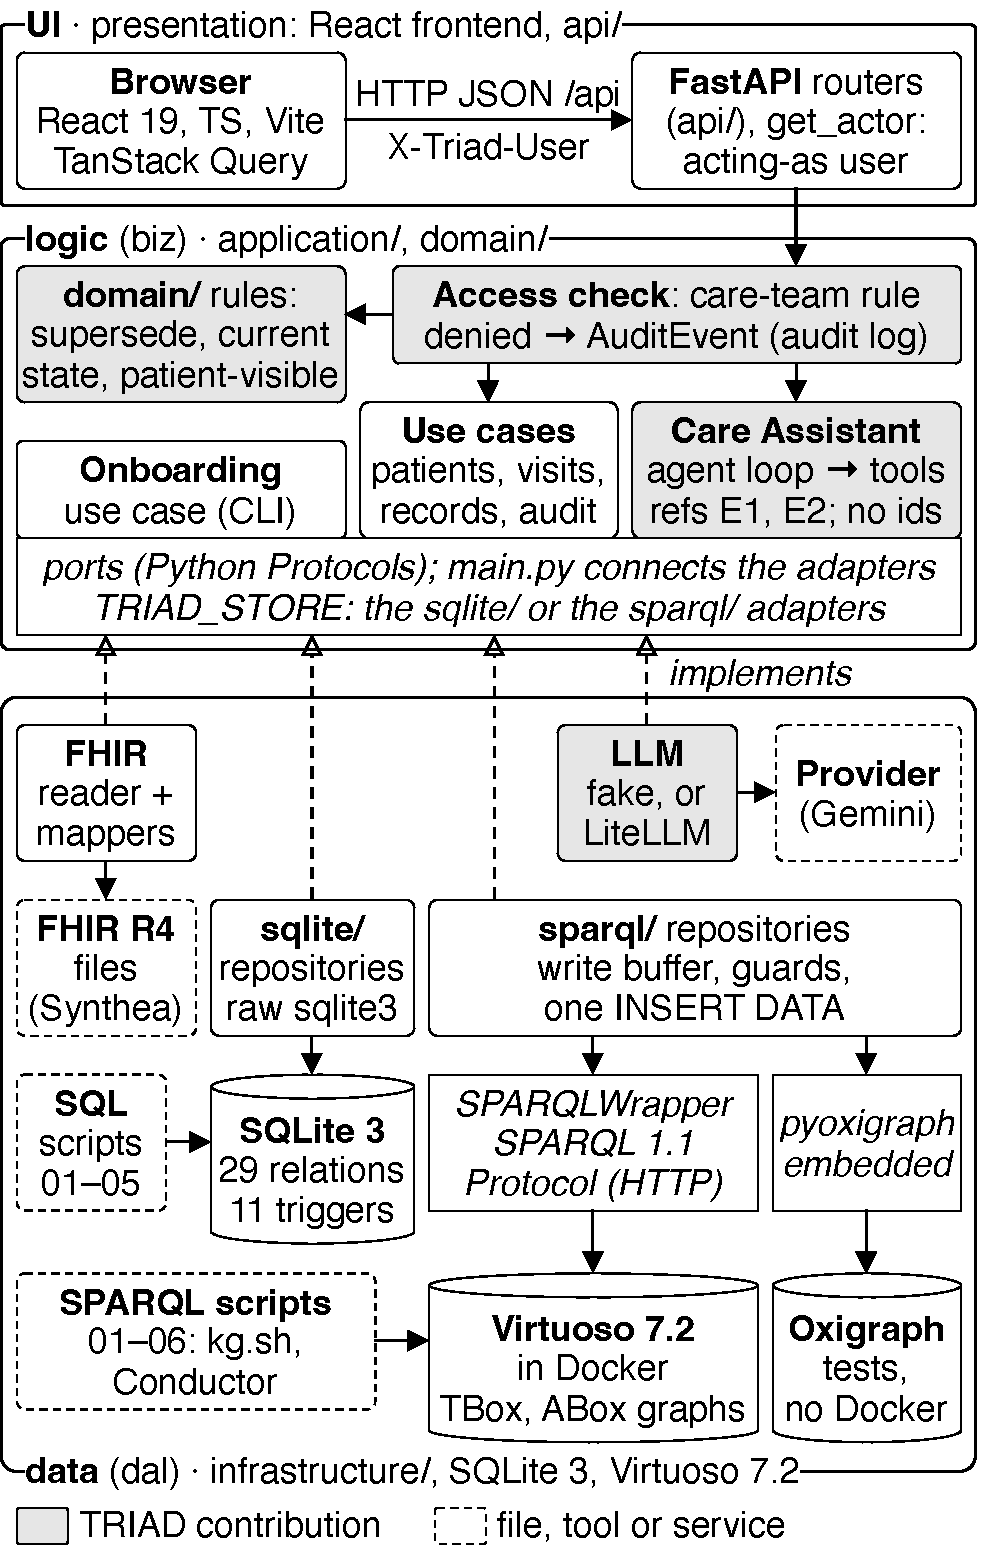
\includegraphics[width=.72\columnwidth]{figures/architecture.pdf}
\caption{Architecture. Grey boxes are TRIAD's contribution.}
\label{fig:arch}
\end{figure}

\section{Architecture and Reproducibility}\label{sec:arch}
Figure~\ref{fig:arch} keeps the three layers of Milestone~4. The \emph{logic} layer talks to ports; \tw{TRIAD\_STORE} selects the SQLite adapters or the SPARQL ones, which buffer the triples of one request, run the guards, and write them in one \tw{INSERT DATA}. \tw{quickstart.sh} starts Virtuoso, builds and loads the graph, runs the fast tests and serves the app; without Docker it uses Oxigraph. On a fresh clone on a second computer, it took about 4.5\,min with Virtuoso the first time (61\,s for the graph) and 2\,min 31\,s the second; with Oxigraph, 2\,min 35\,s. Without Virtuoso, 1,649 backend tests passed and one only went over its time limit (a care-team search took 0.94\,s for 0.9\,s; the rows were correct, so accuracy and design are unaffected); the 561 Virtuoso tests passed, and the 21 browser tests pass on all three stores. The manual path also works: in Conductor we uploaded \tw{triad.owl} and the seed graph and ran scripts \tw{02}--\tw{04}; an \tw{INSERT} is refused (SR619) until \tw{kg.sh init} grants the write.

\section{AI Use and Critique}\label{sec:ai}
From our design and under our review, Claude Code~\cite{claudecode} implemented most of the ontology, mapping, adapters and tests; \tw{doc/ai\_review\_log.md} records each phase. Claude also helped draft this report; we checked every number. (1)~It said its new \tw{assertedBy} fixed our earlier review point that the patient's own 2019 claim is credited to the MOA who typed it. It does not: \tw{assertedBy} copies the message's sender, so it still names the MOA; the point stays open (PROV-O \tw{actedOnBehalfOf} could fix it). (2)~It kept \tw{hasKey} on (name, dateOfBirth) without saying that a reasoner would merge two patients; SHACL rejects the duplicate, but only we stated the risk. (3)~It called the graph OWL~2 DL, but its 31 \tw{xsd:date} values are outside the OWL~2 datatype map. (4)~Its documents kept a stale count (1,298,807 triples). (5)~It presented the new staff rule as converted. (6)~Its Protégé test compares triples, so it fails on a Protégé re-save that has the same axioms. (7)~Two of its agents wired \tw{validate-kg} differently; a test with a fake module missed it. Overall, it was reliable on our design and overclaimed where it judged its own work.


\clearpage
\onecolumn
\raggedbottom
\section*{The Ontology, the Mapping and the App}
\footnotesize

\smallskip\noindent
\begin{minipage}[t]{.17\textwidth}\vspace{0pt}\centering
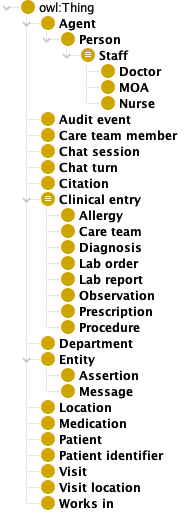
\includegraphics[width=\linewidth]{figures/protege_class_hierarchy.png}
{\captionsetup{justification=raggedright,singlelinecheck=false}\captionof{figure}{The 28 classes in Protégé.}\label{fig:onto}}
\end{minipage}\hfill
\begin{minipage}[t]{.81\textwidth}\vspace{0pt}
\begin{tabularx}{\linewidth}{@{}>{\raggedright\arraybackslash}p{.17\linewidth}>{\raggedright\arraybackslash}p{.25\linewidth}>{\raggedright\arraybackslash}X@{}}
\toprule
\textbf{ER / relational element} & \textbf{OWL construct} & \textbf{Example (Turtle)}\\
\midrule
Entity set & \tw{owl:Class} & \tw{triad:Patient a owl:Class .}\\
Entity (a row) & Named individual; IRI from the surrogate key & \tw{kg:patient/1 a triad:Patient .}\\
Simple attribute & \tw{owl:DatatypeProperty}, functional & \tw{kg:patient/1 triad:name "Elena Marsh" .}\\
Multivalued attribute (Language) & Non-functional property & \tw{kg:staff/2 triad:language "en" , "hi" .}\\
Date / time attribute & \tw{rdfs:Literal} (ontology), \tw{xsd:date} (data) / \tw{xsd:dateTime} & \tw{kg:assertion/3 triad:assertedAt "2026-10-02T11:40:00-04:00"\^{}\^{}xsd:dateTime .}\\
Key & \tw{owl:hasKey} & \tw{triad:Patient owl:hasKey ( triad:name triad:dateOfBirth ) .}\\
Weak entity, partial key & \tw{owl:hasKey} with the owner's inverse & \tw{triad:Assertion owl:hasKey ( triad:inMessage triad:seq ) .}\\
IS-A (disjoint, total) & \tw{rdfs:subClassOf}, \tw{owl:disjointUnionOf} & \tw{triad:Staff owl:disjointUnionOf ( triad:Doctor triad:Nurse triad:MOA ) .}\\
M:1 relationship (foreign key) & Object property, functional, \tw{owl:cardinality 1} & \tw{kg:assertion/3 triad:about kg:clinical-entry/1 .}\\
Identifying relationship & Inverse-functional; =1 on the named inverse & \tw{kg:message/5 triad:contains kg:assertion/3 .}\\
Unary 1:1 (Supersedes) & Functional, inverse-functional, asymmetric, irreflexive & \tw{kg:assertion/3 triad:supersedes kg:assertion/2 .}\\
M:N with attributes & Association class, two functional properties & \tw{kg:works-in/2 triad:ofStaff kg:staff/2 ; triad:atDepartment kg:department/1 .}\\
NOT NULL & \tw{owl:minCardinality 1} (81 restrictions) & \tw{triad:Patient rdfs:subClassOf [ owl:onProperty triad:name ; owl:minCardinality 1 ] .}\\
CHECK \dots\ IN & Closed datatype (\tw{owl:oneOf}) & \tw{triad:intent rdfs:range [ owl:oneOf ( "Report" "Recommendation" "Decision" ) ] .}\\
Authorship & Property chain, PROV-O & \tw{triad:assertedBy owl:propertyChainAxiom ( triad:inMessage triad:issuedBy ) .}\\
\bottomrule
\end{tabularx}

\medskip
\noindent\tw{triad:} = \url{https://github.com/MohamedKhalidmk/TRIAD/ontology/triad\#}; \tw{kg:} = \url{https://github.com/MohamedKhalidmk/TRIAD/kg/} (a query writes the full IRI). The examples use the seed patient Elena Marsh (\tw{kg:patient/1}). Full tables: \tw{src/backend/models/semantic/ontology.md}.
\end{minipage}

\smallskip\noindent
\begin{minipage}{\textwidth}\centering
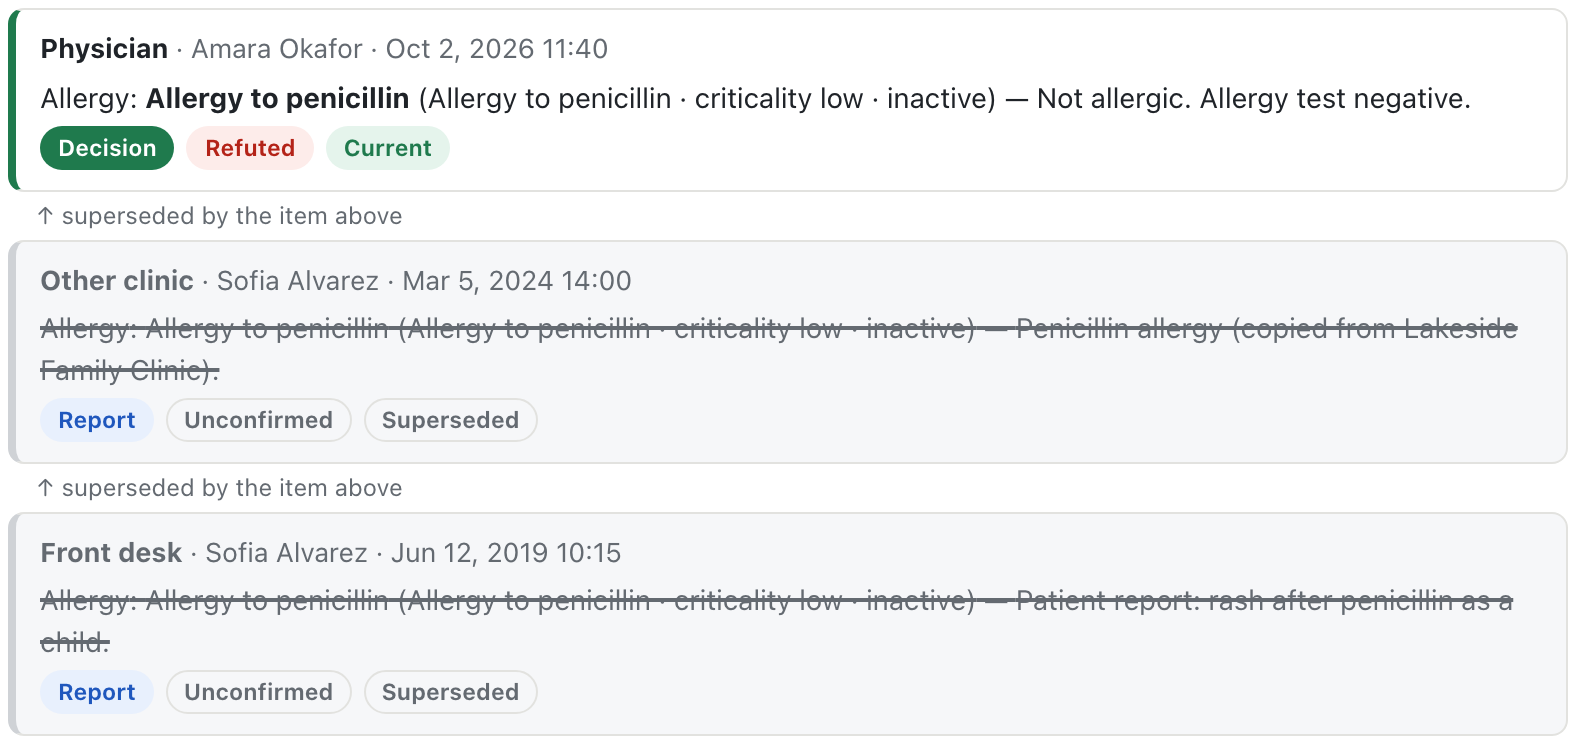
\includegraphics[height=48mm]{figures/app_chain_virtuoso.png}\hspace{5mm}
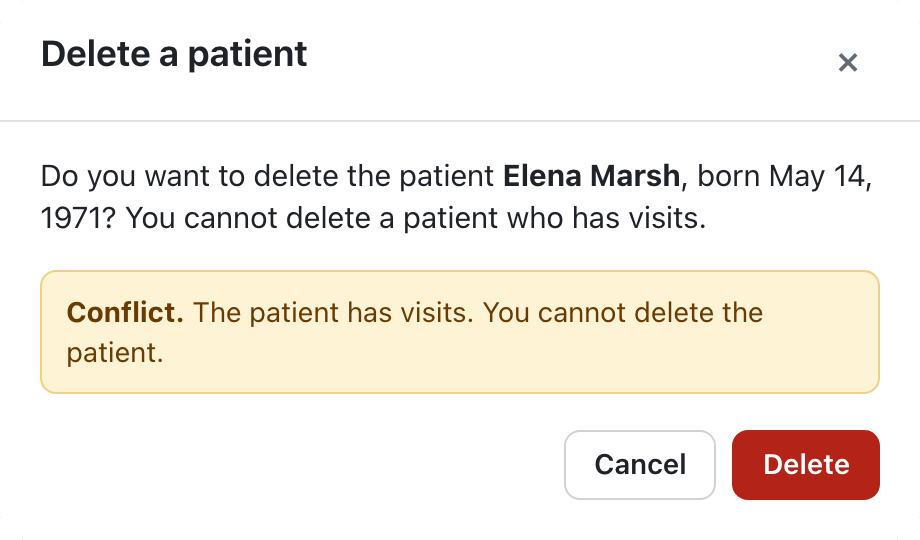
\includegraphics[height=38mm]{figures/app_patient_delete_409.png}
\captionof{figure}{The app on Virtuoso. Left: the penicillin chain (Q2); the 2026 refutation is current, the 2019 and 2024 claims are superseded. Right: \emph{Delete patient} refuses a patient with visits (409, Section~\ref{sec:ops}).}\label{fig:ui}
\end{minipage}


\medskip\normalsize
\begin{multicols}{2}
\bibliographystyle{ACM-Reference-Format}
\bibliography{bibliography}
\end{multicols}
\end{document}
